\section{Concept}
This chapter describes the requirements for the overall concept and goals of this bachelor thesis, analyzes different payment methods to evaluate which meet said requirements and defines a concept and its hardware requirements for a possible implementation.
\\
\subsection{Definition of Prerequisites}

The following prerequisites are required to develop a concept for the sale of electricity between two parties who do not know each other:
\begin{enumerate}
    \item A potential customer Alice owns an electric car and wants to purchase electricity to charge it overnight.
    \item A supplier Bob who owns a smart electrical socket wants to sell electricity.
    \item Alice and Bob do not meet, Alice does not trust Bob to supply the electricity she paid for, Bob does not trust Alice to not wrongfully revert the payment after the electricity has been supplied.
    It has to be assumed that there are bad actors, who want to steal from the other party (in the form of monetary value or electricity).
    \item For all calculations throughout this thesis the following values are assumed:
    \begin{enumerate}
        \item Charging power: 3.7 kW
        \item Electricity price: 0.3 \euro/kWh
        \item Total transferred energy: 40 kWh
        \item Charging duration: 11 hours
        \item Electricity cost: 12 \euro
        \item Price for the customer: 18 \euro{} (profit margin of 50\%)
    \end{enumerate}
\end{enumerate}
\leavevmode
\\
The objective of the next section is to evaluate which payment method is suited best for the described use case.
Thus, the goals of the M2M payment system have to be defined:

\begin{enumerate}
    \item Value has to be transferred from Alice to Bob.
    \item Electricity has to be supplied in return for a payment, whereby the risk or impact of not getting electricity in return has to be minimal.
    \item Alice needs to be able to stop paying for electricity when it is not longer needed, e.g., when the battery is fully charged, without overpaying.
    \item Bob should only start supplying electricity after a valid payment was received and thus the risk of losing electricity is minimized.
    \item Value should be transferred from Alice to Bob at least once per minute to continuously pay for electricity to reduce risk, but transaction fees should stay at a minimum at the same time.
    For this thesis a payment interval of 15 seconds is assumed resulting in 0.007 \euro{} per payment.
    \item All calculations relevant for the payment system should be able to be processed on an embedded platform with low computational power and memory.
\end{enumerate}
\leavevmode
\\
\subsection{Analysis of Different Payment Methods}
In this subsection, the advantages and disadvantages of traditional payment methods, established electronic and online payments and cryptocurrencies are compared and a payment method for the implementation is chosen.
\\
\subsubsection{Traditional Currency}
The simplest form of monetary value is cash, it could be imagined that money could be paid through a coin slot and electricity would be returned as a result.
It's not suitable for this use case, as the risk of not receiving any electricity in return for the customer and the risk of theft for the supplier, e.g., someone violently stealing the cash, is too high.
\\\\
Traditional electronic or online payments like VISA or PayPal pose a low risk of theft for the buyer because of customer protection methods, but the risk for the seller is non-negligible, e.g., in the form of credit card fraud or customer protection exploitation.
Another disadvantage can be seen in the high fees, PayPal, for example, has a pricing of 0.10 \euro{} + 10\% for micro-transactions\cite{paypal-fees} and wouldn't be economically feasible for the predefined goals.
The key strength is a fast, near-instant transaction time.
\\
\subsubsection{Cryptocurrency}
Cryptocurrency payments have some major advantages over the previously analyzed payment methods.
Compared to electronic and online payments, many cryptocurrencies have lower fees and some even work without any fees at all.
Payments can be broken down into fractions, as mentioned above, with payment intervals of a minute or less.
Because all payments are immutable, the supplier has no risk and the customer risks just losing less than one cent for a first payment.
Additionally the currency can be stored right on an embedded device and the machine itself is in charge of sending transactions.
One of the biggest disadvantages of cryptocurrencies for M2M payments are long transaction times, but as the technology is still in its infancy, this might change in the future.
\newpage
Over a thousand different cryptocurrencies exist\cite{coincap} and every one of them has their own rules that can drastically differ from the next one.
Each underlying blockchain technology has their benefits and drawbacks.
In the next paragraphs, some of these digital currencies will be evaluated whether or not they are suitable to reach the set goals.
\\\\\\
\textbf{Bitcoin}\\
Because Bitcoin is the earliest cryptocurrency, it suffers from problems other cryptocurrencies could improve upon.
As demonstrated in Figure \ref{fig:BitcoinConfirmationTime}, scalability is one of these issues.
The block time is 10 minutes\cite{bitcoin-whitepaper} and during peak times the average confirmation time can take more than two hours.
Thus bitcoin should not be considered for this use case.
\\
\begin{figure}[H]
    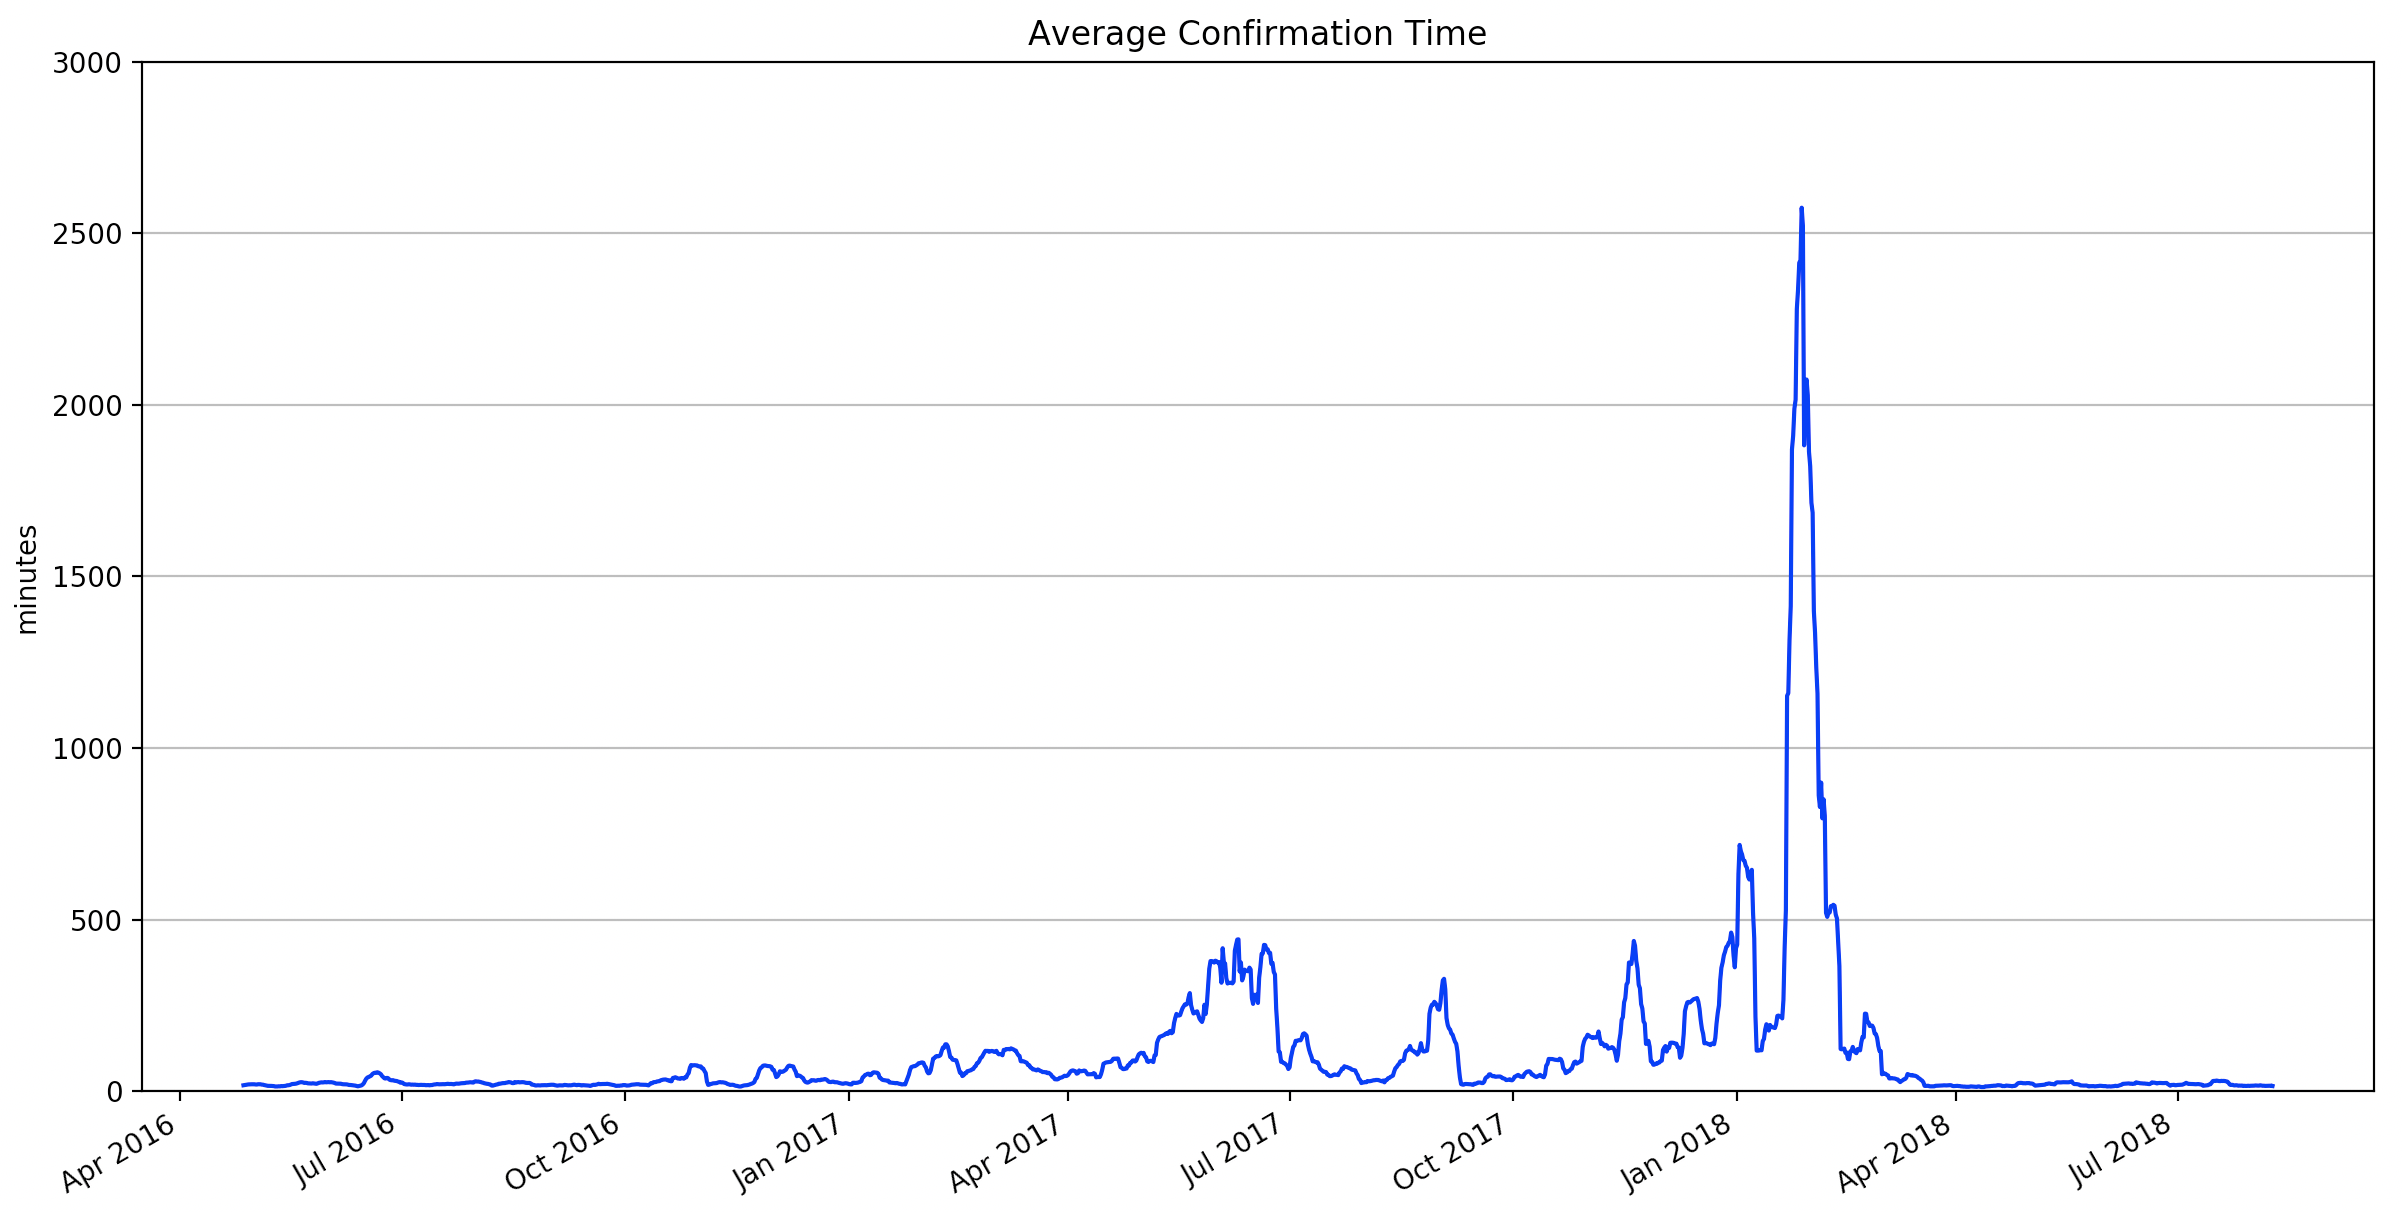
\includegraphics[width=\textwidth]{img/average-confirmation-time.png}
    \caption{Average confirmation time of a transaction on the Bitcoin blockchain\cite{btc-conf-time}}
    \label{fig:BitcoinConfirmationTime}
\end{figure}
\leavevmode
\\
\textbf{IOTA}\\
As previously mentioned, there are some cryptocurrencies that work without any fees that are worth to be considered.
One of these currencies is IOTA.
It was designed especially with M2M payments in mind and the underlying technology, called Tangle, differs from traditional blockchains.
The way it works is that before someone's transaction can be validated, they need to validate other transactions first\cite{tangle}.
In theory, this makes the network scale especially well — the more transactions are broadcasted, the shorter the transaction times get.
In practice, transaction times are at 2.6 minutes at the time of writing\cite{iota-time} and therefore not fast enough for this use case.
\newpage
\textbf{Nano}\\
Another feeless cryptocurrency is called Nano, formerly known as RaiBlocks.
It is built upon a technology called block-lettuce.
Each account on the network is an independent blockchain which can update itself asynchronously from the rest of the accounts.
This makes Nano not only have zero transaction fees but also allows it to have transaction times of less than a second.
It can also handle way more TPS than Bitcoin and Ethereum, namely around 100 TPS over a longer period of time with peaks up to 300 TPS\cite{nano-stress-test}.
\\\\
Unfortunately, at the time of development of the prototype, the Nano network faced some issues which resulted in transaction times in up to 20 seconds, as seen in Figure \ref{fig:NanoConfirmationTime}.
After the V18 update these problems were solved and the transaction times returned back to less than a second\cite{nano-confirmation-time}.
\begin{figure}[H]
    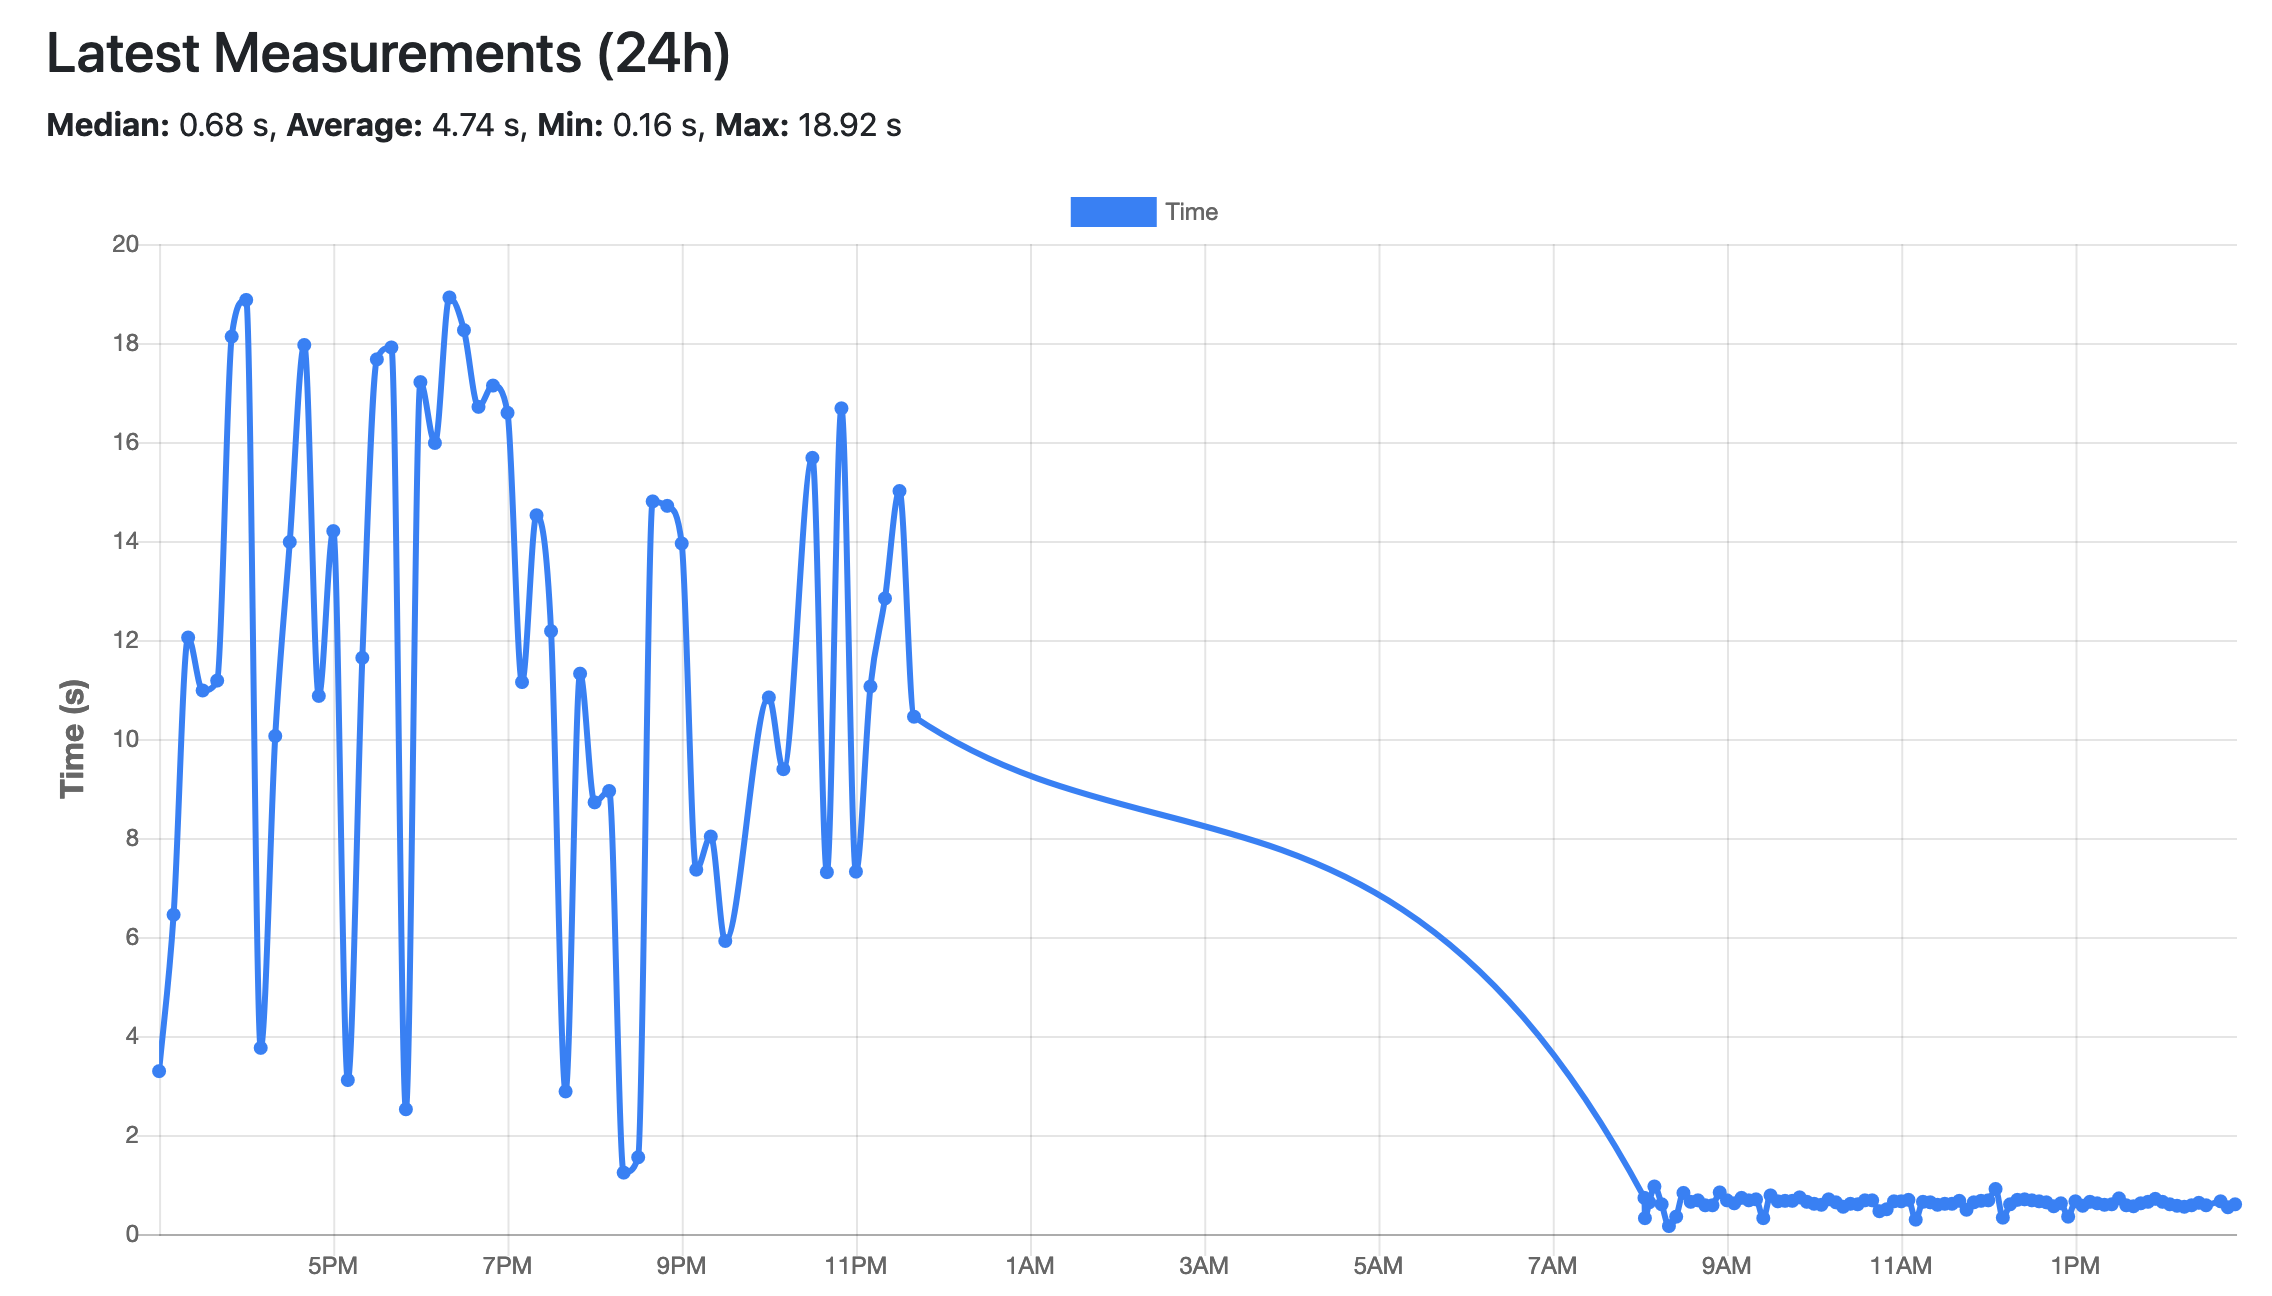
\includegraphics[width=\textwidth]{img/nano-confirmation-time.png}
    \caption{Improvements of transaction times after the update to V18 on Feb. 22nd, 2019\cite{nano-confirmation-time}}
    \label{fig:NanoConfirmationTime}
\end{figure}
Although the currency was considered at first, the main reason Nano was not chosen for the implementation is that it was not built with M2M transactions in mind.
To prevent spamming, i.e., attacking the network through congesting it with transactions, PoW needs to be generated in order to send or receive transactions.
According to the Nano white paper\cite{nano-white-paper} an Intel Core i7-4790K processor with 4.00 GHz can handle up to 0.33 TPS.
A microcontroller would not be able to generate the PoW required for the transactions in a reasonable amount of time.
Instead, a dedicated server would be required for each supplier and customer, which would store the private keys and handle the transmission and reception of transactions.
The micro controllers would merely communicate with said servers and therefore the currency did not meet the defined requirements.
\newpage
\textbf{Ethereum}\\
Ethereum has a block time of 15 seconds.
At the time of writing the fee to be included in the next block is 0.01 \euro\cite{ethereum-fee}.
In this case, the transaction would be fast enough to meet the goal of 4 transactions per minute, but the transaction fees would exceed the payment, raising the total price as much as 143\%.
\\\\
One way to cut transaction fees is the use of off-chain transactions.
As previously mentioned, these work very similarly to on-chain transactions: information like a beneficiary and value can be signed by a sender, so it can be proven where the transaction originates from.
They differ from each other, as off-chain transactions are not recorded on the blockchain.
They can be sent from one participant to another directly, therefore there is no transaction fee or transaction time involved.
A number of these off-chain transactions can be bundled in a payment channel.
In the end, these transactions have to be settled on the blockchain, actually modifying the ledger and updating the balances of all participants.
Thus, the 2,460 transactions required during a charging period of 11 hours can be bundled into a few transactions on the blockchain.
Sending on- and off-chain transaction requires computations like encoding, hashing or signing of data which can be achieved on an embedded platform.
Therefore this payment method meets all the requirements listed above.
\\\\
Ethereum was chosen for the implementation of this prototype, as it implements a virtual machine with the ability to execute code, therefore a payment channel can be built using smart contracts.
The following steps briefly explain how the payment concept works:
\\
\begin{enumerate}
    \item The customer places a deposit (max. purchase value) into the smart contract and initializes the payment channel.
    \item The customer signs an off-chain transaction and sends it to the supplier.
    \item Once the supplier receives the transaction, the delivery of electricity begins.
    Steps 2 \& 3 are repeated until the customer or the supplier want to discontinue the exchange.
    \item As soon as any party wants to close the payment channel, the supplier submits the off-chain transactions to the smart contract.
    Each party is now able to withdraw their share from the smart contract.
\end{enumerate}
\begin{figure}[H]
  \begin{center}
    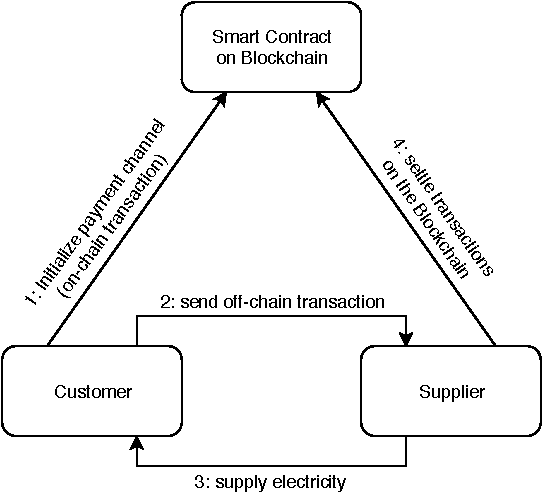
\includegraphics[height=8cm]{img/payment_channel.pdf}
    \caption{Sketch of a payment channel}
    \label{fig:paymentchannel}
  \end{center}
\end{figure}
With payment channels, the risk of the supplier is minimal, as electricity must only be provided when a valid payment was received.
The customer only risks losing one transaction for the initialization of the payment channel and one off-chain transaction if no electricity is provided in return.
\\\\
In total, only 4 on-chain transactions have to be made.
One for the payment channel initialization, one for the settlement, and one by each party to withdraw the balances, totaling all transaction fees at a couple cents.
\newpage
\subsection{Component Requirements}
As demonstrated in Figure \ref{fig:concept} the concept is based on four components.
A supplier, a customer, a node in form of a server and a smart contract on the Ethereum blockchain.
\\
\begin{figure}[H]
  \begin{center}
    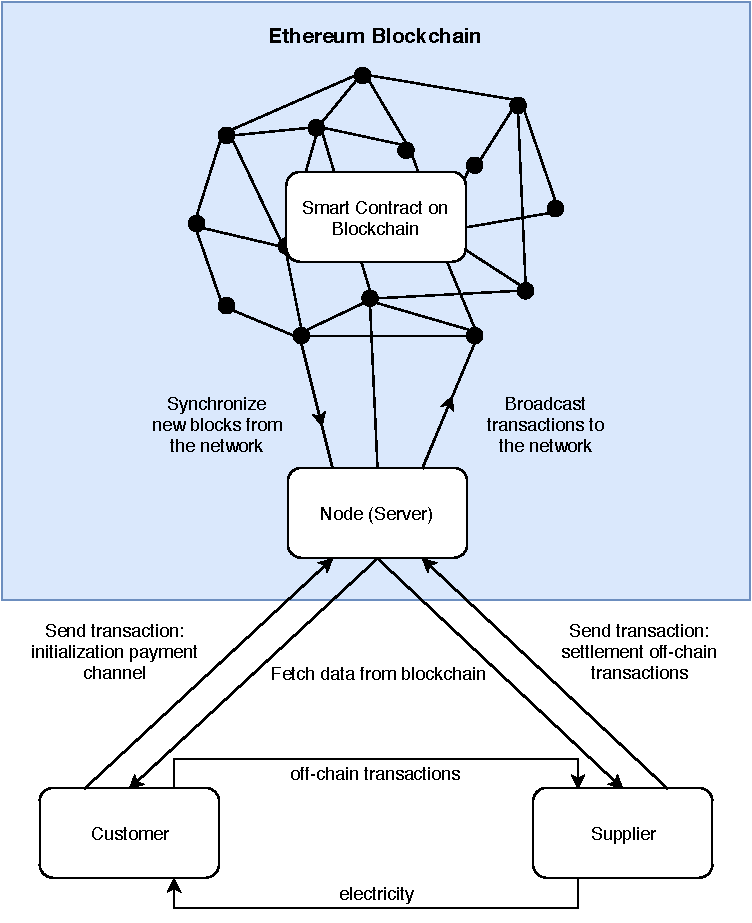
\includegraphics[height=17cm]{img/concept.pdf}
    \caption{Sketch of the concept}
    \label{fig:concept}
  \end{center}
\end{figure}

The supplier should have a microcontroller which is integrated directly into an electrical socket.
This way it can be powered directly by the supplier's circuit and can be protected against external damages, e.g., caused by weather or human influences.
A relay should be placed between the circuit and the socket, which can be switched on and off by the microcontroller to start and stop the supply of electricity to the customer.
For the communication with the Ethereum network an internet connection is required.
It can be either established by connecting to a cellular network using a SIM card or to a WiFi network, preferably of the supplier itself.
\\\\
The customer should have a microcontroller which is integrated into an electrical plug.
If it is integrated into a short extension cord, any electrical device can be connected to it and be charged.
The microcontroller should be able to measure whether electricity is flowing through the cord using a current sensor, e.g., a hall effect-based sensor.
The plug is required to communicate with the Ethereum network as well, therefore a SIM card can be integrated to connect to a cellular network or the plug can use the supplier's WiFi connection for the communication.
The microcontroller can be powered directly by the supplier's socket itself, as the electricity output can be limited to sufficiently power the customer's microcontroller but not enough to charge any device.
\\\\
Both parties are required to communicate with each other, as payment information needs to be exchanged and off-chain transactions need to be sent and received.
The microcontrollers can send information to each other over the circuit itself using \abbr{power-line communication}{PLC} or, if the customer and supplier are using the same WiFi network, it can be used to handle the communication between both parties.
\\\\
The design and functionality of the off-chain transactions is defined by the implementation of the smart contract, which should have the following features.
It should act in the interest of the customer and the supplier, securing both parties from fraud.
A payment channel should be initialized by the customer by depositing an amount of Ether into the smart contract.
The smart contract should act as a trustee, managing the funds until the payment channel is closed again.
The customer can then start signing off-chain transactions with its private key and sending them to the supplier.
When the payment channel is ready to be closed, the supplier should submit the off-chain transactions to the smart contract, as it is in its interest to submit all transactions.
The smart contract is required to verify whether the off-chain transactions were indeed signed by the customer.
If the transactions are valid, the smart contract can then pay out the total transaction volume to the supplier and refund the remainder to the customer.
To ensure that both parties are protected, the payment channel should have an expiration date.
In case the supplier fails to submit a valid signature in a certain amount of time, the customer should be able to withdraw the entire deposit from the smart contract.
\\\\
To initialize and close the payment channel, the customer and the supplier need to be able to communicate with the Ethereum blockchain, which is achieved with a node.
It is the only component required to run on a server, as the entire blockchain history has to be downloaded which takes up several gigabytes of data.
When relevant payment information, e.g., the price per second stored in the smart contract, needs to be fetched from the blockchain, the server sends the information stored in its synchronized local copy.
When data is sent to the blockchain in form of a transaction, the entire process of generating the transaction computes on the microcontroller.
The transaction is then sent to the node which forwards it to the other blockchain participants.
Therefore, the node acts as a gateway between the Ethereum network and the microcontrollers.
\\
\subsection{Risks \& Concerns}
Although choosing payment channels implemented on a blockchain over traditional payment methods brings some advantages in low transaction fees and every party being in charge of their own money, there are some drawbacks that are worth noting:
\\\\
The reason no party has to trust another when using smart contracts is immutability.
Once the code has been deployed to the blockchain, it cannot be changed after the fact.
This poses a risk, as bugs found in the smart contract code cannot be fixed either.
This already resulted in losses of multiple hundreds of millions of dollars on the Ethereum blockchain alone\cite{dao-hack}.
\\
As soon as funds are stored inside a smart contract or on a physical device there is a financial incentive for hackers to try to steal the money.
As the private keys of the customer and supplier are stored on the embedded devices themselves, every part of the microcontroller has to be carefully secured, so under no circumstances the private key can be extracted to steal funds.
Therefore, PLC should be chosen over a WiFi connection for the communication between the customer and the supplier.
\\
Because the concept is designed as a P2P, middleman free system, not only 3rd parties have an incentive to steal funds.
If the customer uses the supplier's WiFi network to communicate with the blockchain, a man in the middle attack should be prevented by using a HTTPS connection secured over TLS.
\\
Transactions are the most secure part of the concept, as they are always digitally signed.
Therefore, even if they are intercepted by a malicious actor, they can only be used for their intended purpose.
\\\\
Another concern is that the concept would not work economically at the time of writing.
Cryptocurrencies and the blockchain technology are still in its infancy and therefore the price is extremely volatile.
A sudden rise or drop of 40\% in price is not rare and would heavily influence the customer experience.
Additionally, only very few people actually own cryptocurrencies and are willing to pay or receive payments using cryptocurrencies.
Because of the low adoption rate, the concept would not be economically feasible as a real product at the time of writing.
\newpage
\subsection{State of the Art}
The exploratory research conducted for this thesis focused on studying concepts and design choices of similar projects completed in the commercial field.
\\\\
A few companies already started researching and experimenting with blockchain technologies and even went as far as combining it with e-mobility.
A company called accessec GmbH built a prototype of a car wallet that works with the IOTA cryptocurrency and integrates a point of sale allowing to conduct transactions with vendors seamlessly\cite{car-wallet}.
Bosch teamed up with the energy supplier EnBW to build a prototype of a blockchain based charging station\cite{bosch-dlt}.
\\\\
The project that came closest to the topic of this bachelor thesis is called Share\&Charge, formerly known as Blockcharge\cite{share-charge}\cite{blockcharge}, which was founded by Innogy, a subsidiary of the energy company RWE\cite{innogy}.
It launched at the end of April 2017 with close to 1,500 charging stations, but the project was closed merely a year later\cite{share-charge-closed}.
It claimed to be a P2P charging network calling itself the "AirBnB of Charging Stations".
It was running on the Ethereum mainnet where anyone could become a charging station owner by purchasing a smart electrical socket to sell electricity.
At first glance it seemed like the solution to this thesis' question, but upon further investigation the decentralization aspect had to be questioned.
The electrical socket was communicating with a smartphone app to manage the purchase of electricity.
This app had to be preloaded with fiat currency via PayPal, etc., the transaction was conducted in fiat and a charging station owner could only withdraw fiat currency as well.
There is no evidence that the monetary transaction itself was handled on the blockchain and not just the record aspect of it.
Additionally, it was claimed that the system worked without a middleman but the fee that had to be paid to Share\&Charge with every charging process contradicts that claim.
All this information led to the conclusion that the private keys probably were not handled by the users themselves which is a crucial point in building decentralized applications.
\\\\
To summarize, all projects combining blockchain with e-mobility seem to be bringing existing centralized business models to the blockchain and could work just as well with traditional payment methods.
Furthermore, no technical information, let alone source code, could be found that could be used or improved upon for this bachelor thesis.
